\documentclass[11pt,letterpaper]{article}
\usepackage[utf8]{inputenc} %Codificacion del texto (ISO Latin1 encoding)

\usepackage{fancyhdr} %Permite acomodar a tu gusto la parte de arriba y
\usepackage[spanish]{babel} %Permite definir el idioma del dcumento
\usepackage{graphicx} %Permite exportar imagenes en formato eps
\usepackage{url} %Tipo de fuente para correos y paginas
\usepackage{hyperref}
\usepackage{pgf}
\usepackage{fleqn}
\usepackage{amssymb}
\usepackage{fancyvrb}
\usepackage{sectsty}
\usepackage{makeidx}
\usepackage{colortbl} %Permite colocar colores a las tablas
\usepackage{booktabs}
%Margenes%
\parskip 1mm %Espacio entre parrafos

\setlength{\topmargin}{0pt}

\oddsidemargin	0.5cm  % Ancho Letter 21,59cm
\evensidemargin 0.5cm  % Alto  Letter 27,81cm
\textwidth	15.5cm
\textheight	21.0cm
\headsep	4 mm
\parindent	0.5cm
\pagestyle{fancyplain}
\lhead{Informática y Sociedad} %Parte superior izquierda
\rhead{\bf \it Informe Final} %Parte superior derecha
\lfoot{\it Influencia de las tecnologías de la información en colaboraciones
internacionales }
\cfoot{} %Parte inferior central
\rfoot{\bf \thepage} %Parte inferior derecha
\renewcommand{\footrulewidth}{0.4pt} %Linea de separacion inferior

\newtheorem{theorem}{Theorem}
\newtheorem{acknowledgement}[theorem]{Acknowledgement}
\newtheorem{algorithm}[theorem]{Algorithm}
\newtheorem{axiom}[theorem]{Axiom}
\newtheorem{case}[theorem]{Case}
\newtheorem{claim}[theorem]{Claim}
\newtheorem{conclusion}[theorem]{Conclusion}
\newtheorem{condition}[theorem]{Condition}
\newtheorem{conjecture}[theorem]{Conjecture}
\newtheorem{corollary}[theorem]{Corollary}
\newtheorem{criterion}[theorem]{Criterion}
\newtheorem{definition}[theorem]{Definition}
\newtheorem{example}[theorem]{Example}
\newtheorem{exercise}[theorem]{Exercise}
\newtheorem{lemma}[theorem]{Lemma}
\newtheorem{notation}[theorem]{Notation}
\newtheorem{problem}[theorem]{Problem}
\newtheorem{proposition}[theorem]{Proposition}
\newtheorem{remark}[theorem]{Remark}
\newtheorem{solution}[theorem]{Solution}
\newtheorem{summary}[theorem]{Summary}
\newenvironment{proof}[1][Proof]{\noindent\textbf{#1.} }{\ \rule{0.5em}{0.5em}}

\newcommand{\primaria}[1]{
	\textbf{\underline{#1}}
}

\newcommand{\foranea}[1]{
	\textbf{\textsl{#1}}
}

\newcommand{\primyfor}[1]{
	\underline{\foranea{#1}}
}

\makeatletter
\newcommand\subsubsubsection{\@startsection {paragraph}{1}{\z@}%
                                   {-3.5ex \@plus -1ex \@minus -.2ex}%
                                   {1.5ex \@plus.2ex}%
                                   {\normalfont\bfseries}}
\newcommand\subsubsubsubsection{\@startsection {subparagraph}{1}{\z@}%
                                   {-3.5ex \@plus -1ex \@minus -.2ex}%
                                   {1.5ex \@plus.2ex}%
                                   {\normalfont\bfseries}}


\makeatother
%\makeindex
\bibliographystyle{plain}

\begin{document}

%%%%%%%%%%%%%%%%%%%%%%%%%%
%Definicion de la portada%
%%%%%%%%%%%%%%%%%%%%%%%%%%
\begin{titlepage}
    \begin{center}
	%\begin{tabular}{ccc}
	\begin{tabular}{c}
		
\includegraphics[width=0.9\textwidth]{img/logos}
		
	   % 
\includegraphics[width=3cm]{img/utfsm}
	   % & 
	   % \hspace{-0.2cm}
	   % \begin{tabular}{c}
	   % Universidad Técnica Federico Santa María \\ \hline
	   % \vspace{0.2cm}
	   % Departamento de Informática\\
	   % \vspace{1.2cm}
	   % \end{tabular}
	   % \hspace{0.2cm}
	   % &
        %    
\includegraphics[width=2cm]{img/di}
	\end{tabular}

	\vspace{4cm}
	%Titulo del Documento
	\begin{tabular}{c}
		\vspace{3cm}
		\Large{\sc{Seminario de Modelos y Métodos Cuantitativos}}\\
		\huge{\sc{Tarea 2}}\\\\
		%\includegraphics[scale=0.7]{img/portada} \\\\
	\end{tabular}

    \vspace{5cm}
	\begin{tabular}{lr}
			\textbf{Alumnos} & \\
							 & \\
         	\normalsize{Cristián Maureira Fredes} & \url{cmaureir@csrg.inf.utfsm.cl}\\
         	\normalsize{Gabriel Zamora Nelson} & \url{gzamora@csrg.inf.utfsm.cl}\\

							 & \\
			\textbf{Profesor} & \\
							 & \\
         	\normalsize{Andrés Moreira} & \url{amoreira@inf.utfsm.cl}\\
	\end{tabular}

\vspace{2cm}

	%Fecha
    \normalsize{\sc{\today}}\\
    %\normalsize \textbf{Fecha de Entrega:} & {14 de Noviembre del 2010}\\
    \end{center}
\end{titlepage}

\tableofcontents
\newpage

\section{Introducción}
\label{sec:introduccion}
\frame
{
\frametitle{Introducción}
\begin{itemize}
	\item Motivación del problema.
	\item Sobre la técnica.
	\item Implementación inicial.
	\item Sintonización.
	\item \blue{Control}.
	\item Resultados.
\end{itemize}
}



\section{Antecedentes}
\label{sec:antecedentes}
\subsection{Público Objetivo}

\subsubsection{Descripción}
El público objetivo para el presente estudio, se compone principalmente
por personas que se encuentren realizando proyectos de carácter internacional, 
los cuales debido a su distribución geográfica, no les permite una comunicación
relativamente fluida. Además de verse forzosamente necesitados de medios de
comunicación para suplir la distancia. Por otro lado, el no presentar
importancia el área de dichos proyectos e idioma en que se lleve a cabo.

\subsubsection{Información existente}
% Estube buscando alguna publicación/página que hable de la cultura
% americana/alemana, pero no he logrado encontrar nada util =/.

%sobre las herramientas para el trabajo colaboratio
Existen organizaciones que ya han experimentado con herramientas para el
trabajo colaborativo en linea para mejorar la fluidez del intercambio de la
información entre todos sus miembros~\cite{herramientas_trabajo_colaborativo}.
Uno de estas es el uso de wikis. Las wikis~\cite{wikis} son sitios web cuyas
páginas pueden ser editadas por múltiples personas desde un navegador web,
permitiendo redactar documentos colectivamente, siendo ampliamente usadas hoy
en día. El caso más emblemático es el de la wikipedia\cite{wikipedia},
enciclopedia virtual para compartir el conocimiento, editada por voluntarios
de todas las partes del mundo.
Algunos de los softwares más utilizados para ello son
MediaWiki~\cite{mediawiki}, MoinMoin~\cite{moinmoin} y Twiki~\cite{twiki}.
Otros tipos de herramientas utilizadas para la coordinación de diferentes equipos
de trabajo son las herramientas de Software Configuration Management
(SCM~\cite{scm}). Normalmente son utilizadas en actividades de desarrollo de
software, y permiten tratar y controlar la elaboración de código fuente por
varios desarrolladores simultáneamente, pudiendo realizar un seguimiento del
estado de las versiones y sus cambios. Algunas de las herramientas más utilizadas para
esto son Git~\cite{git}, un sistema de control de versiones distribuido,
Subversion (SVN~\cite{svn}), un sistema de control de versiones centralizado,
y  Trac~\cite{trac}, sistema que integra una wiki y sistemas de control de
versiones como Git y SVN, y posee múltiples plugins~\cite{plugin} para
extenderle nuevas funcionalidades.



\subsection{Dominio de la Investigación}

\subsubsection{Descripción}
Con respecto al dominio de la presente investigación, son dos distintas
instancias donde personas de Estados Unidos, Alemania y Chile se reunen
a discutir temáticas en relación al proyecto ALMA:

\begin{itemize}
	\item ACS Weekly Meeting: Reunión donde asisten los colaboradores
(desarrolladores) más importantes del proyecto ALMA, la cual es coordinada
 desde Garching, Alemania.
	\item OSF Coordination Meeting: Reunión en la cual acuden personas de Nuevo
México (EEUU), Garching (Alemania) y Valparaíso (Chile), la cual es 
coordinada por los representantes del grupo ALMA-UTFSM. En ella se plantean temas
de interés general.
\end{itemize}

El dominio de investigación trata sobre que será medido en el corto y largo plazo, 
con respecto a la influencia que tienen las tecnologías de la información en la forma
de trabajo mencionado anteriormente. Se tratará de enfocar los resultados en relación
a objetivos a corto plazo como lo son estados de avances en tareas específicas, para 
medir en que manera influyen las tics en una comunicación de avances de manera fluida e 
intercultural. A largo plazo se medirá a nivel de colaboración el grado de cohesión que 
estas organizaciones logran gracias a la influencia de las tics, refiriéndonos a cantidad
de proyectos logrados con éxito y creación de instancias colaborativas.

\subsubsection{Información existente}

A nuestra investigación le interesan los temas de la comunicación y las
relaciones interpersonales. El dominio es bastante amplio, desde el estudio de
la comunicación oral y corporal la construcción de las relaciones
interpersonales que forman a los grupos de trabajo tanto como las tecnologías
existentes para suplir o complementar a los medios de comunicación.
Dentro de estos ámbitos, existen investigaciones\cite{obs_collaborative} que
han concluido dentro de la información transmitida en las comunicaciones
interpersonales, el lenguaje corporal, el uso de gestos, manos y la forma en
cada persona gesticula transmite significativa información adicional, y cómo
el espacio en el cual se están comunicando influye en las relaciones de
trabajo.

En el trabajo colaborativo desarrollado entre diferentes grupos separados
geográficamente, el tipo de visibilidad que halla de los demás, el moverse
dentro del mismo ambiente compartido, el estar presentes al mismo tiempo, la
audibilidad, tangibilidad y simultaneidad son claramente diferentes al estar
limitados a la comunicación utilizando los medios que las tecnologías nos
ofrecen para ello. Como afecta cada uno de estos factores a la forma de
organización y la forma de trabajo a desarrollar ha sido
estudiada~\cite{proximity_collaboration} concluyendo que, aunque las personas
presentan una mayor facilidad para relacionarse en ambientes de proximidad
física, es posible para las personas colaborar a través de la distancia,
usando cualquier tecnología que tengan disponible. Las personas son capaces de
adaptarse a los medios que disponen, con cierto grado de aceptación, para poder
lograr la comunicar lo que desean. Además, se concluye que el medio de
comunicación utilizado cambia la naturaleza de la comunicación y la naturaleza
de la comunicación, pudiendo pasar de una comunicación menos social a una
enfocada a los tópicos a tratar.

Hoy en día los ambientes de trabajo en el mundo laboral no son lo mismo que
hace años atrás. Tradicionalmente los empresarios han organizado el trabajo de
forma centralizada, sin importar del tipo de trabajo llevado a cabo por cada
uno de los miembros de la empresa. Ahora, la tendencia es la descentralización
e individualización de las diferentes funciones desarrolladas, refiriéndose
con ello a la división de las funciones en los individuos de un grupo de
trabajo, a la delegación y la subdivisión de las diferentes tareas a
realizar por una empresa.
Por ello, mantener una comunicación fluida que evite la pérdida de
identificación de cada trabajador con los objetivos de la empresa o grupo de
trabajo se vuelve de suma importancia.
Para poder evitar estas situaciones, se espera encontrar similitudes que
permitan mejorar las falencias de los modelos de trabajo y la distanciación de
sus identidades con la del grupo de trabajo\cite{trabajo_flexible}.

También se cuenta con la experiencia vivida por el grupo ALMA-UTFSM durante
su formación y desarrollo\cite{utfsm_alma}, en donde se analiza los cambios
que experimentó durante la maduración de su modelo organizacional, donde las
tecnologías de la información determinaron en gran medida las formas de
trabajo colaborativas llevadas a cabo. Se destacan las variables del ambiente
que lograron alcanzar el éxito del grupo, las cuales se deben analizar en
conjunto para entender la real importancia de cada una de ellas. El tener estudiantes
entusiastas y motivados, seleccionados tanto por sus habilidades sociales como
técnicas, y un grupo docente involucrado, que les guía y da soporte, permite
que se fomente la proactividad y que los proyectos estén en
continuo desarrollo.



\section{Análisis y Resultados de Antecedentes}
\label{sec:analisis}
Se describen a continuación los análisis a distintos factores que hemos
decidido como equipo, que son dignos de estudiar.

\subsection{Idioma}
Es conocido que el idioma universal, nos guste o no,
es el inglés, por lo tanto al momento de participar en
cualquier reunión con personas de distintos países,
la única solución es poder comunicarnos con dicho lenguaje.

Por lo tanto cada miembro presente, debe preocuparse no tanto
por saber la traducción de palabras en español al inglés,
sino en algo mucho más complejo, saber expresar las ideas
en un lenguaje distinto que el idioma del país natal.

%Agregar más

\subsection{Zonas Horarias}
Si bien es cierto, para cualquier persona, fijar una reunión
a una cierta hora no es una tarea difícil, tenemos que darnos
cuenta que al momento de pensar en una reunión internacional,
la mayoría de los países poseen una zona horaria distinta, por
lo cual, las personas encargadas tanto de organizar como de
participar en alguna reunión de esa índole, debe poseer el
conocimiento del horario de los países en cuestión,
y saber cuantas horas de diferencia se tienen, pues, mientras
en un lugar el día puede estar comenzando, el otro, puede estar
acabando.

Actualmente en dichas reuniones, uno de los mayores problemas
que se han tenido, son las diferencias muy grandes entre EEUU, 
Alemania y Chile, pues si tomamos en consideración a Chile,
EEUU tiene 2 horas menos y Alemania tiene 6 horas más, lo cual
claramente es un problema, pues se necesita encontrar un balance.
%Agregar más

\subsection{Costumbres}
Es conocido de que lamentablemente en Chile, nos caracterizamos
por ser un poco impuntuales, independiente de si se trata de una
reunión formal, a una fiesta de cumpleaños. Por lo que debido a lo
anteriormente señalado, en todos los países hay distintas costumbres
y es en la puntualidad que nos hemos fijado, en el cual Alemania
destaca por cumplir su palabra completamente, pues al momento
de iniciar una reunión, si es a las 11:00 am, no es ni un par
de minutos antes ni un par de minutos después, pero lamentablemente
tanto en EEUU como en Chile, ocurre lo contrario.

Es por lo anteriormente señalado que cada vez que se comienza una
reunión ocurren los problemas de ``Estamos esperando a una persona
para poder comenzar.''

\subsection{Experiencia Técnica}
Si bien es cierto, expresar las ideas en otro idioma, no es algo
trivial que se le dé innatamente a cualquier persona, para participar
en distintas reuniones donde se discuten temáticas de una índole técnica
es necesario tener el conocimiento técnico necesario para, aparte de
entender la idea que la otra persona está queriendo expresar, entender
que significa lo que está diciendo.
Es por ésto, que las personas que participan en las reuniones,
es gente que conoce lo que es ACS (ALMA Common Software) a un nivel
intermedio, para poder sobrevivir en un lugar donde se discutan ideas
en torno al dicho software.
%Agregar más

\subsection{Medios de comunicación}
Cuando uno realiza teleconferencias con distintas personas,
nunca al finalizar, quedan todas las ideas completamente claras,
o mirado desde otro punto de vista, siempre hay nuevos temas
o dudas respecto a lo que se habló, por lo cual es necesario
comunicarse con las personas que plantearon dicha idea, o que
simplemente están a cargo.

Para poder realizar una comunicación más fluida entonces,
es necesario tener otros medios para poder comunicarnos,
es decir, aparte de Skype~\cite{Skype} para realizar
dichas teleconferencias, se necesitan otras formas, como lo son:
\begin{itemize}
   \item Mensajería Instantánea: Es necesario establecer un protocolo de comunicación
		único para dicho objetivo, en el cual se pueda agregar a las personas de interés, logrando
		una interacción rápida y expedita. En nuestro caso se utiliza Yahoo Messenger.
   \item Correo Electrónico: Si bien es cierto existen las reuniones, es necesario también
		poder tener una comunicación un poco indirecta para comentar problemas, o presentar
		avances de un cierto trabajo a todas las personas interesadas mediante listas de correo.
   \item Acceso Telefónico: Las reuniones se realizan mediante teleconferencias, por lo cual
		es necesario tener acceso telefónico con el extranjero, o en el caso nuestro, poder
		contar con una cuenta Skype para llamadas a todo el mundo.
\end{itemize}

\subsection{Medios de almacenamiento de información}
Para cada reunión apropiadamente desarrollada,
es necesario poseer una minuta para tener un orden
cronológico de los temas a tratar o el orden
en que las personas tienen la palabra, para poder
expresar sus ideas y consultas.

Por lo tanto es muy positivo, que todas las personas
estén familiarizadas con dichos medios, en este caso hablamos
de TWiki (referencia a la TWiki), un medio de almacenamiento
comunitario de comunicación, que es utilizado tanto como para
presentar las minutas, como para el desarrollo de los distintos
proyectos colaborativos alrededor de lo que es ACS.

%Agregar mas

\subsection{Relación con Tecnologías de la Información}

Si nos damos cuenta, en todos los puntos señalados anteriormente
la tecnología juega un papel fundamental, ya sea desde el
almacenamiento de información, como para una comunicación directa.

% Agregar mas


% Secciones nuevas
\section{Estudio de Campo}
\label{sec:estudio}
% Obtención de datos a partir de una muestra del “público objetivo”,
% 	para conocer la relación de éste con el
%	tema tecnológico que se está estudiando.
%
% Observaciones:
%   a) Se puede aplicar diferentes técnicas de obtención de datos:
%	   encuesta, entrevista, focus groups, observación participante, etc.
%
%	   IMPORTANTE: obtener registros audiovisuales (fotos, videos, etc)
%
%   b) El tamaño de la muestra (cantidad de público objetivo), debe ser
%		estimada numéricamente, para que la investigación tenga validez científica.
%
Tomando en cuenta que el presente trabajo conlleva un análisis a el impacto de tecnología
en las colaboraciones internacionales de nuestra universidad, el poder recolectar información
audiovisual como fotos y videos es imposible, debido a que las mayorías de las reuniones son
con personas fuera del país, por lo cual el único material que se presenta es con respecto a
las reuniones acá en la Universidad.

La obtención de datos se realizó a partir del análisis de las reuniones mencionadas anteriormente,
donde se evaluaron los siguientes aspectos:
\begin{itemize}
	% Saber lo que es una teleconferencia, como se usa, cuando hay un error, saber lo que pudo probocarlo
	% Conocer como se realizan las conferencias, como llamar a la gente, como conectarse, etc.
	\item Entendimiento de conceptos tecnológicos.
	% Conocer skype, twiki, lenguajes de programación.
	\item Entendimiento de herramientas tecnológicas.
	% Cuantas veces alguien pide "repetir" lo ultimo que se dijo,
	%  tener la capacidad de explicar conceptos o situaciones técnicas en otros idiomas.
	\item Problemas con el idioma.
	% Que nos dejen hablar y participar en las reuniones
	\item Respeto con todos los colaboradores.
	\item Integración con el equipo de trabajo.
	\item Participación en otros proyectos ya iniciados.
	\item Ayuda sobre proyectos.
	\item Medios de comunicación.
\end{itemize}

Los datos acerca de los puntos anteriores son valores promedios, para los numéricos
y los más frecuentes en caso de ser cualitativos.

\subsection{Encuesta}
La presente encuesta se encuentra disponible en~\footnote{Encuesta Realizada - \url{http://csrg.inf.utfsm.cl/~cmaureir/encuesta.html}},
y los resultados presentados son hasta el \emph{5 de Julio del 2010}~\footnote{Resultados Encuesta - \url{http://csrg.inf.utfsm.cl/~cmaureir/resultados.pdf}}
\begin{enumerate}
    \item ¿Ha trabajo remotamente con otros grupos de trabajo?\\
        R: | Si | No
    \item ¿En promedio, cuantas personas conformaban el grupo trabajo?\\
        R:\\
            | menos de 3\\
            | entre 3 y 5\\
            | entre 6 y 8\\
            | entre 8 y 12\\
            | 12 +
    \item ¿En promedio, cuanto es el tiempo de duración de los
    proyectos o trabajos?\\
        R:\\
            | menos de 1 Mes\\
            | entre 1 y 2 Meses\\
            | entre 3 y 4 Meses\\
            | entre 5 y 10 Meses\\
            | menos de 1 Año\\
            | entre 1 y 2 Años\\
            | más de 2 Años
    % Preguntar por forma de trabajo, jerarquías, etc.
    \item ¿Encuentra que trabajar remotamente beneficia el trabajo en
        equipo?\\
        R: | Si | No
    \item Tecnologías de la Información
    \begin{enumerate}
        \item ¿Cuales de éstas herramientas ha utilizado para trabajar y
            comunicarse remotamente?\\
        R:\\
           | Skype\\
           | Wiki's (Twiki, Mediawiki)\\
           | Aplicaciones web de Manejo de Proyectos (Ej:Trac, Redmine)\\
           | Llamadas telefónicas\\
           | Teleconferencia\\
           | Otra:

        \item ¿Encuentra necesario el uso de tecnologías de la información
        para comunicarse?\\
        R: | Si | No

    \end{enumerate}
    \item Dificultades
    \begin{enumerate}
        \item ¿Ha experimentado problemas de comunicación con el uso de tecnologías?\\
        %\item ¿El idioma ha significado un problema para la comunicación de las partes?
        R: | Si | No
        \item Si es así, seleccione las problemáticas más comunes que ha
        encontrado:\\
        R:\\
	    | Se pide comúnmente que se "repita" lo ultimo que se dijo.\\
	    | Dificultad para explicar o transmitir conceptos o situaciones técnicas.\\
        | Fallas técnicas.\\
        | Otras: 
        \item ¿Lograron solucionar éstos problemas?\\
        R: | Si | No
        \item Si es que pudo, ¿De que manera lo logro?\\
        R:\\
        | Usando otras tecnologías.\\
        | Otra manera:
        \item ¿Considera que el uso de tecnologías mantiene el respeto entre los participantes?\\
        R: | Si | No
        \item ¿Cree que la integridad entre equipos de trabajo se ve afectada negativamente, al sólo tener disponible tecnologías en vez de una comunicación directa?\\
        R: | Si | No
        \item ¿Se ha integrado a equipos de trabajo donde debe en el camino aprender a utilizar tecnologías?\\
        R: | Si | No
        \item Si es así, ¿le ha sido fácil?:\\
        R: | Si | No\\
	\end{enumerate}
    % Cosas que faltan por evaluar:
	%\item Participación en otros proyectos ya iniciados.
\end{enumerate}

\subsection{Resultados}
La presente encuesta fue realizada a personas pertenecientes al estudiantado
de la universidad UTFSM y a miembros del equipo de desarrollo de ALMA-UTFSM
residentes en Chile, EEUU y Alemania.

Total de Personas encuestadas 29 personas.
Se muestran a continuación los resultados de la encuesta, representados en
gráficos de barras para cada pregunta y las respuestas correspondientes a
ella.

\begin{center}
	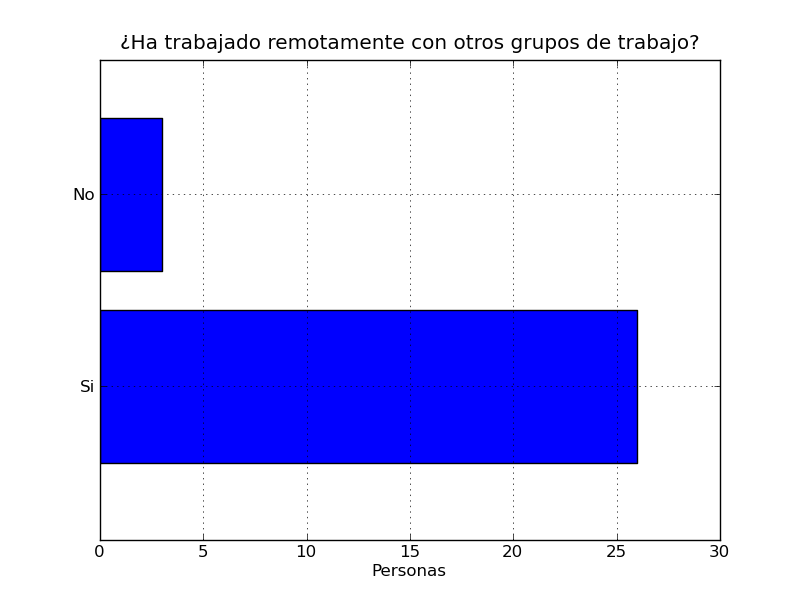
\includegraphics[width=0.8\textwidth]{images/fig1}\\
	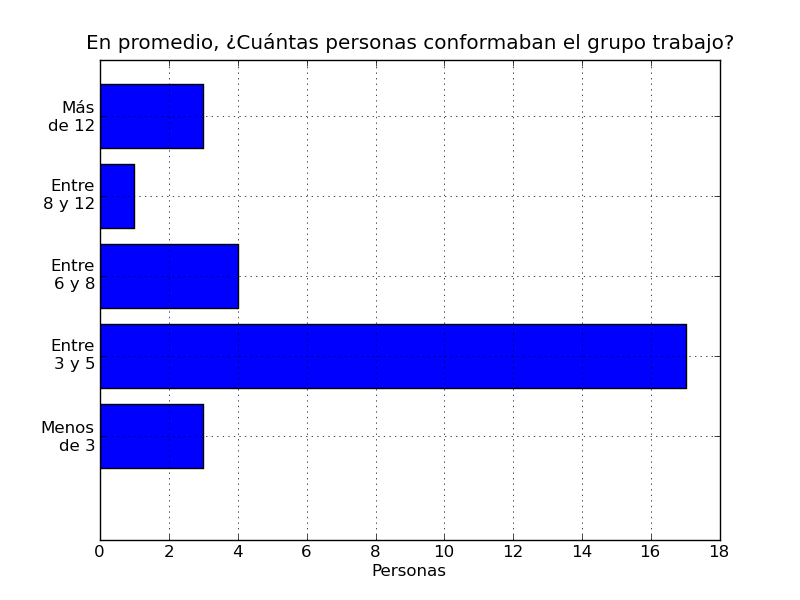
\includegraphics[width=0.8\textwidth]{images/fig2}\\
	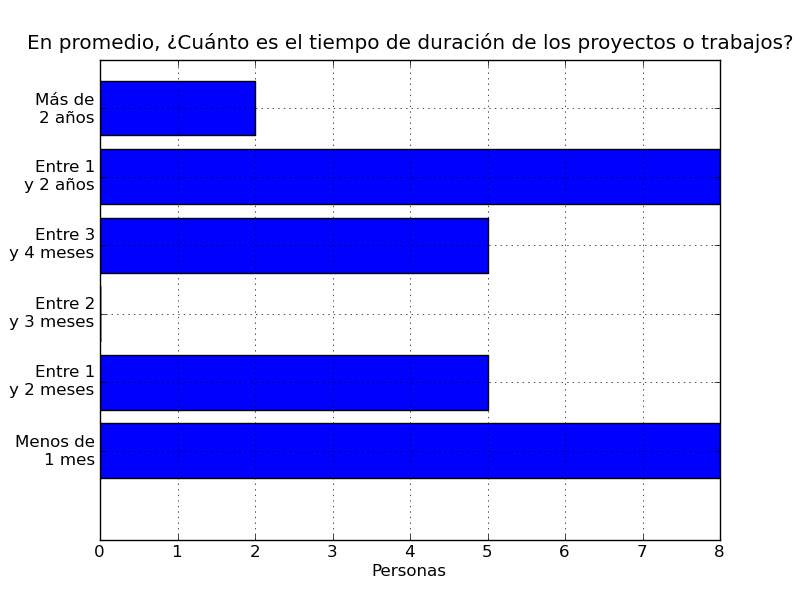
\includegraphics[width=0.8\textwidth]{images/fig3}\\
	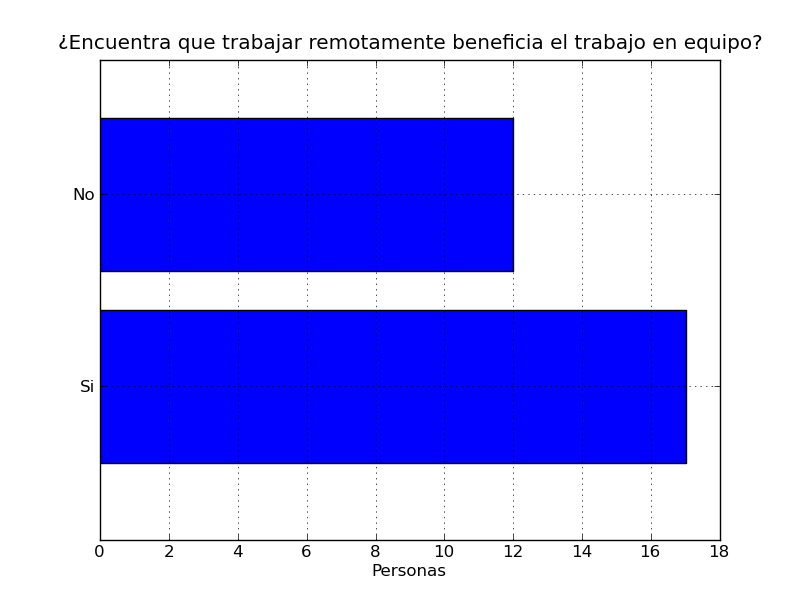
\includegraphics[width=0.8\textwidth]{images/fig4}\\
	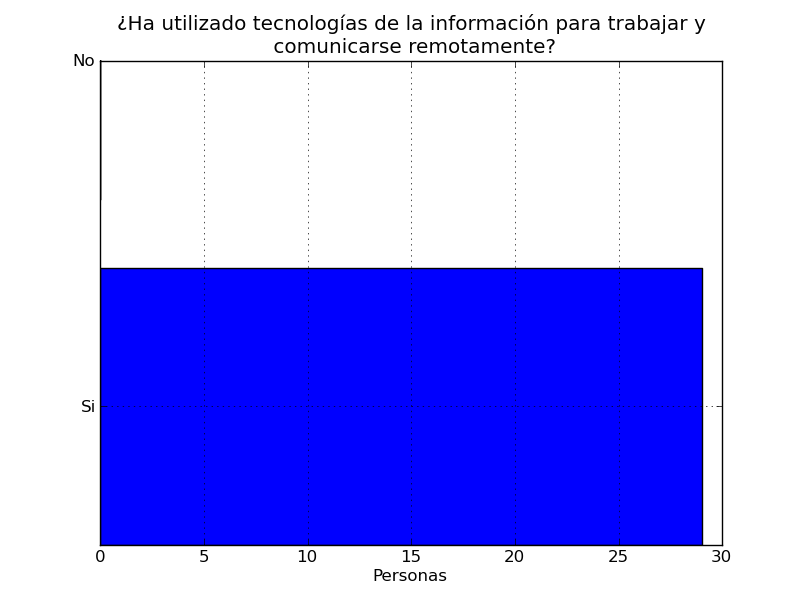
\includegraphics[width=0.8\textwidth]{images/fig5}\\
	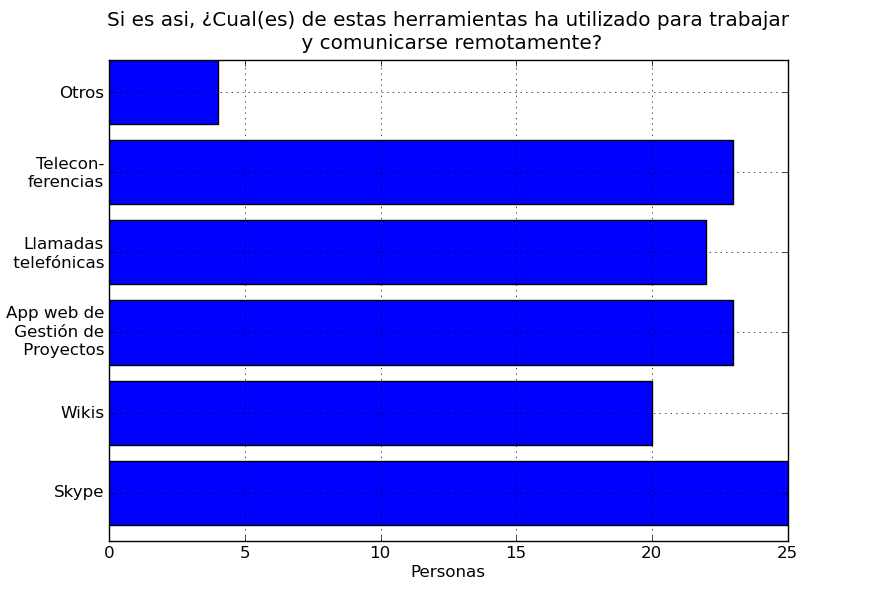
\includegraphics[width=0.8\textwidth]{images/fig6}\\
	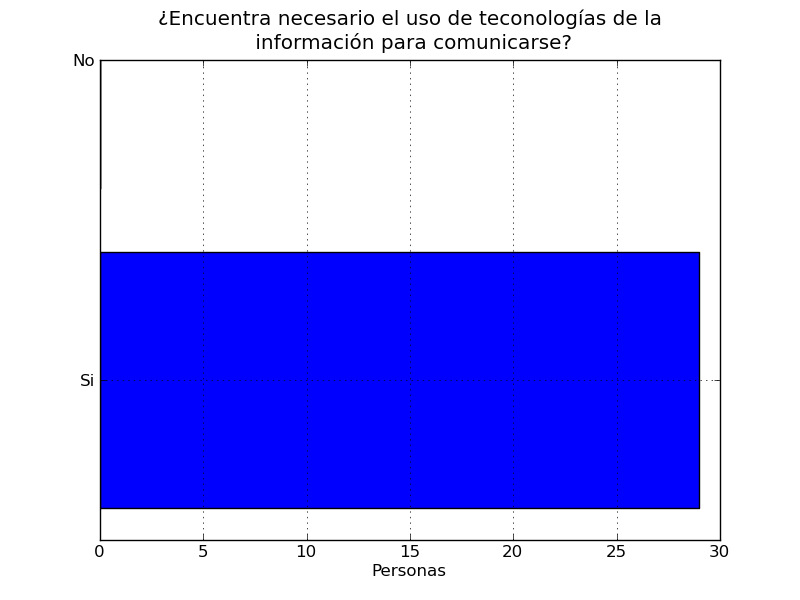
\includegraphics[width=0.8\textwidth]{images/fig7}\\
	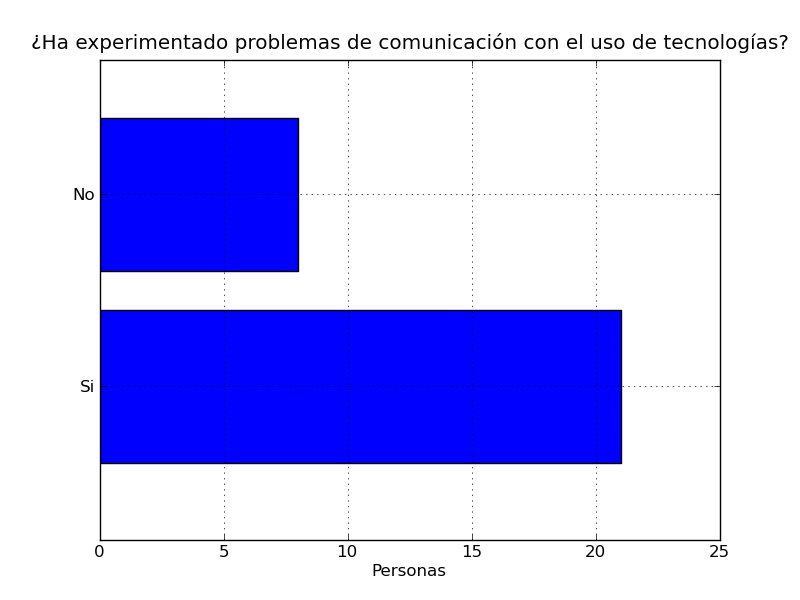
\includegraphics[width=0.8\textwidth]{images/fig8}\\
	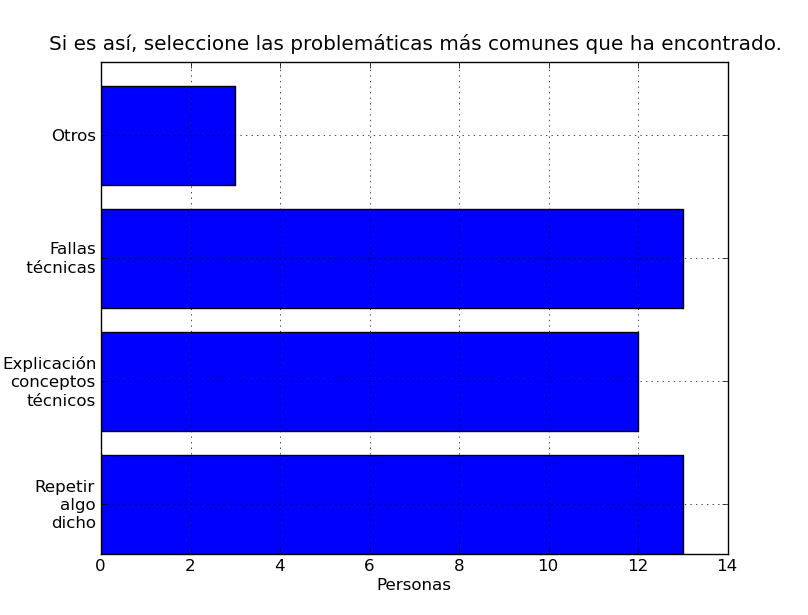
\includegraphics[width=0.8\textwidth]{images/fig9}\\
	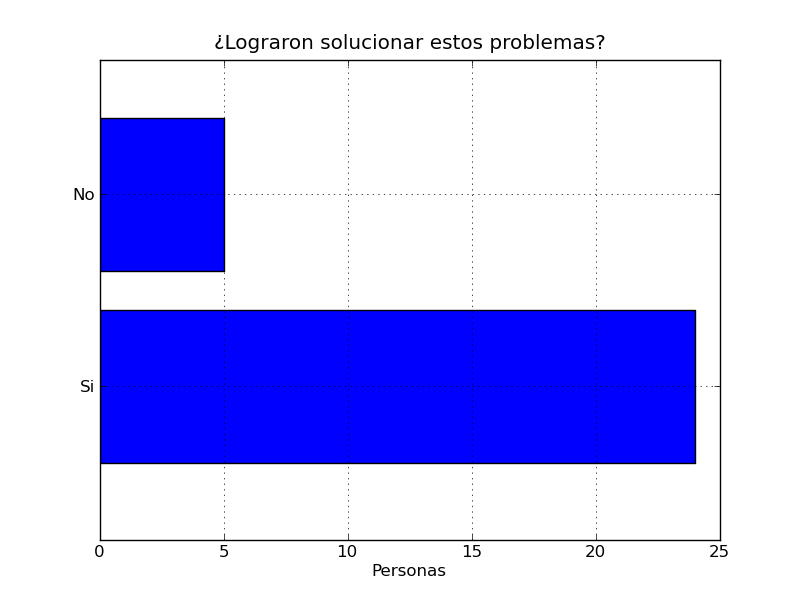
\includegraphics[width=0.8\textwidth]{images/fig10}\\
	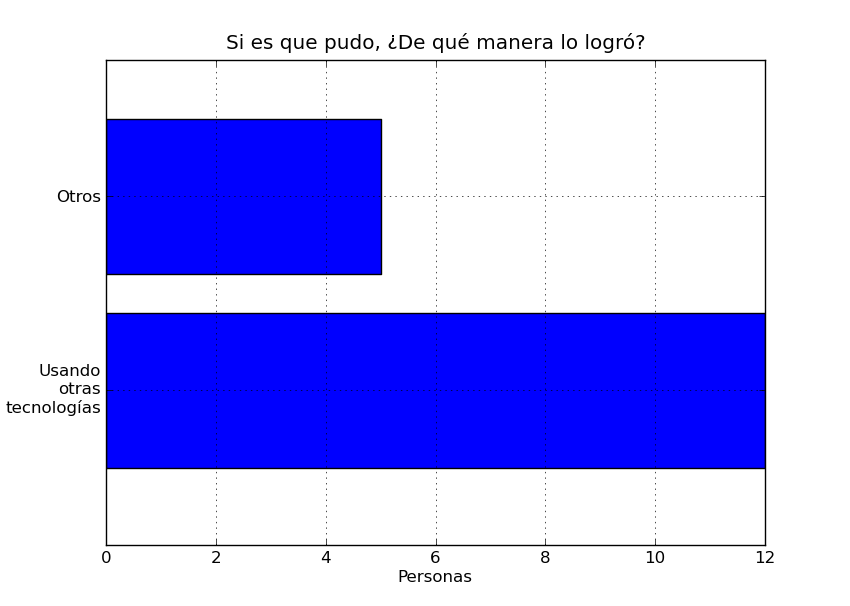
\includegraphics[width=0.8\textwidth]{images/fig11}\\
	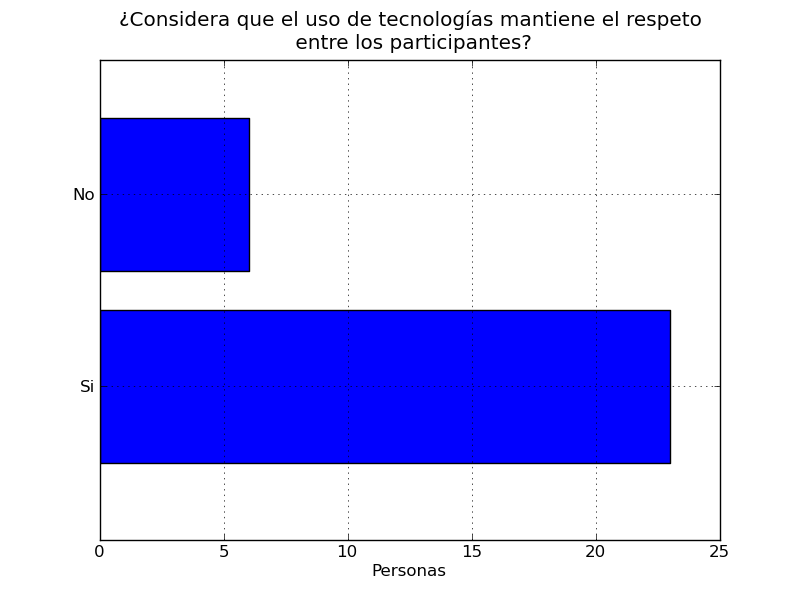
\includegraphics[width=0.8\textwidth]{images/fig12}\\
	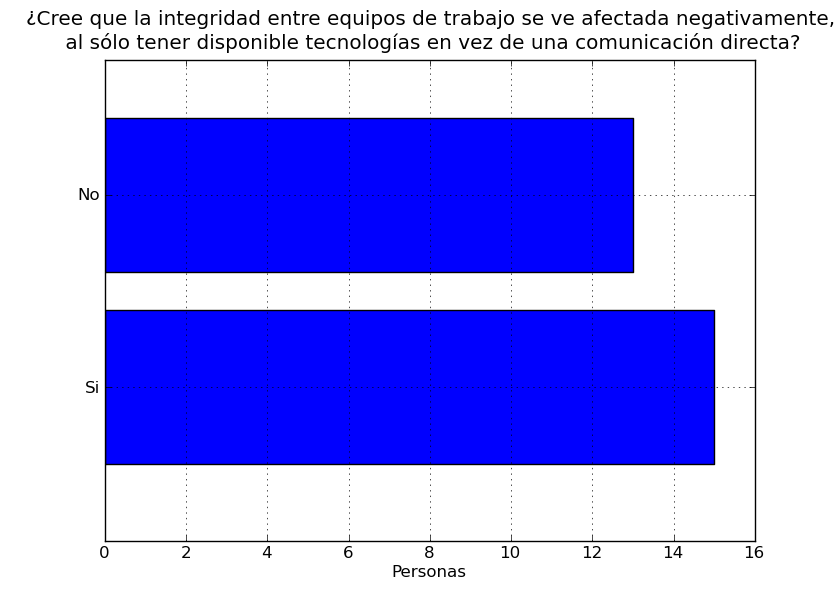
\includegraphics[width=0.8\textwidth]{images/fig13}\\
	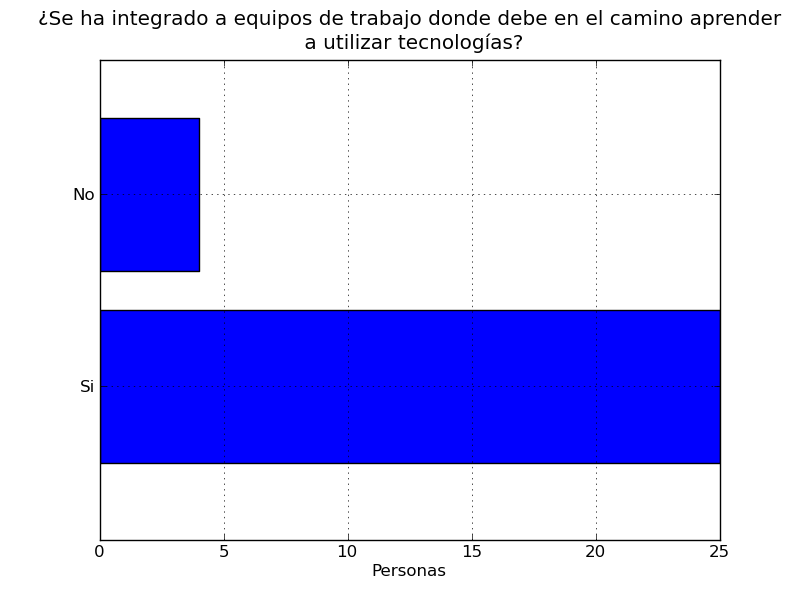
\includegraphics[width=0.8\textwidth]{images/fig14}\\
	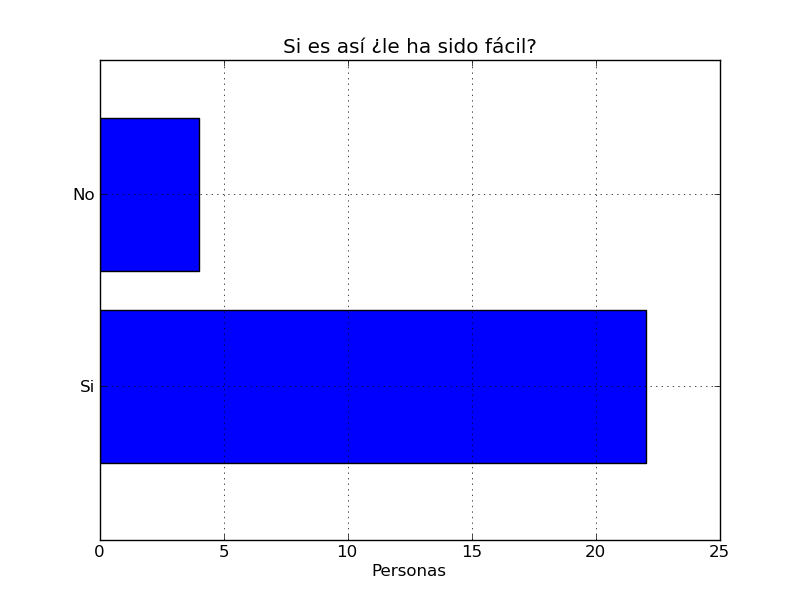
\includegraphics[width=0.8\textwidth]{images/fig15}
\end{center}

El análisis a los presentes resultados es explicado en la siguiente sección.


\section{Análisis de la relación entre ``público objetivo'' y ``tema tecnológico''}
\label{sec:relacion}
% Analisis de la relacion entre publico objetivo y tema tecnologico
% 
% A partir de los datos obtenidos en el Estudio de Campo, uds.
%  deberan analizar los datos cuantitativos y cualitativos del
%  publico objetivo, para determinar los impactos del tema
%  tecnologico con relación al publico objetivo

La herramienta más utilizada entre los encuestados resultó ser de mensajería
instantánea y de videoconferencia (Skype), pasando en segundo lugar a las
llamadas telefónicas y teleconferencias. La preferencia por Skype se puede
comprender a causa de que las tarifas asociadas al servicio de llamadas
internacionales posee un costo muy menor en comparación con los servicios de
telefonía convencional. Un lugar importante fue abarcado por las aplicaciones
de gestión de proyectos y Wiki's, las cuales se puede concluir que son de
alguna forma necesarias por el tipo de proyectos que los encuestados realizan,
que requieren de una buena documentación y detalle de las tareas realizadas
por cada miembro. Todos encuentran necesario el uso de tecnologías para
comunicarse, y todos han tenido experiencias con al menos una de ellas en su
trabajo.

Entre algunas de las respuestas a las problemáticas más comunes al comunicarse
a través de las tecnologías, se nombró el hecho de que las personas no
llegaban a la hora de la reunión. Éste hecho puede ser un problema
considerable, ya que si la reunión se hacen de forma remota, las personas de
una u otra localidad normalmente desconocen las causas del retraso, generando
situaciones de estrés y pérdidas de tiempo de desarrollo de los proyectos. De
todas formas, ese tipo de problemas se puede considerar ajeno a las
tecnologías, siendo inherente a las personas con las que uno trabaje.
Otra problemática que era independiente de las tecnologías que se utilizaran,
pero propia de los trabajos con personas de diferentes países, eran las
diferencias culturales de cada persona. Éstas pueden ser solucionadas a
través de una buena comunicación, realizando reuniones presenciales cada
cierto tiempo para mejorar los lazos entre cada uno y así poder comprender más
las diferencias de cada uno. De todas formas, una cantidad considerable se
encontró con fallas técnicas a la hora de comunicarse, pero la mayoría logró
superarlas profundizando su conocimiento del uso de las herramientas o
cambiando las tecnologías utilizadas. Considerando que las personas
encuestadas poseen un alto nivel técnico, estas soluciones puede que no tengan
la misma efectividad para grupos de trabajo de todo tipo.

Se puede apreciar como la mayoría de los problemas de comunicación eran por
dificultades de idioma, en donde lo común era que se necesitara repetir lo
último dicho, junto con una dificultad para explicar y/o transmitir conceptos,
lo cual se dificulta al no poder utilizar la comunicación no verbal para
expresarse. La mayoría de los encuestados comparten la opinión de que es
necesario el uso de tecnologías para comunicarse hoy en día. 

La mayoría de los encuestados han tenido que integrarse a equipos de trabajo
sin presentar grandes dificultades para aprender nuevas tecnologías. Las
tendencias indican que éstas cada vez son más utilizadas, y las habilidades de
adaptación a las mismas son cada vez mayores, especialmente por el hecho que
las personas desde cada vez más temprano empiezan a interactuar con las
tecnologías de la información, ya sea en la escuela o en sus casas. El
problema normalmente se encuentra con las personas vivieron el proceso de
tecnocratización de los medios de comunicación en una edad más temprana, y
presentan por ello una mayor dificultad o rechazo hacia las nuevas
tecnologías.

En general se concuerda que las tecnologías son imparciales a la hora de
mantener el respeto entre los integrantes, pero dependiendo de que herramienta
se esté utilizando, al disminuir los canales de comunicación, aumentan las
probabilidades de que sucedan interpretaciones erróneas sobre lo que se
intenta comunicar, pudiendo provocar roces innecesarios entre los integrantes
más sensibles del equipo. Por ello, a veces es bueno abstenerse de realizar
recomendaciones, dichos o bromas que puedan ser malentendidas estando fuera de
contexto.


\section{Resultados}
\label{sec:resultados}
%El analisis de los datos obtenidos,
%	arrojara resultados que uds. deberan presentar en esta seccion.
%	Deben poner enfasis a los impactos del tema tecnologico en el
%	publico objetivo, y sus proyecciones.

En la sección anterior, pudimos darnos cuentas de los resultados de la encuesta realizada a personas que trabajan
en el mismo ambiente que se presenta en el trabajo, dándonos cuenta cuales herramientas utilizaban, si les eran útiles, etc,
pero ahora nos queremos enfocar en los \emph{impactos} principalmente, de nuestro tema principal, en el las personas estudiadas.

Con respecto a las tecnologías, podemos profundizar mucho acerca del proceso de \emph{selección}, \emph{desarrollo} y su propio \emph{uso},
y sobre todo, en el análisis a los impactos producidos por cada uno de los factores anteriormente señalados.
Éstos impactos, no influyen sólo en la persona, sino que van más allá, poseen una suerte de influencia en el quehacer humano y por ende
todo lo que lo rodea, \emph{alterando} su comportamiento.

Analizando uno de los investigadores más importantes en ésta área, McLuhan~\cite{mcluhan}, podemos obtener ciertas preguntas que nos van a servir para ver el impacto
de las tecnologías en nuestro ambiente.
Las preguntas son:
\begin{itemize}
	\item ¿Qué genera, crea o posibilita?
	\item ¿Qué preserva o aumenta?
 	\item ¿Qué recupera o revaloriza?
	\item ¿Qué reemplaza o deja obsoleto?
\end{itemize}

Las cuales debemos resolver por cada tecnología que se quiera evaluar.

Si consideramos las \emph{tecnologías de la información} como un elemento tecnológico, podemos pasar a responder dichas preguntas para el trabajo en general:
\begin{itemize}
	\item \emph{¿Qué genera, crea o posibilita?}\\
		Gracias a las tecnologías de la información, estamos generando nuevos caminos de comunicación para realizar determinadas actividades en cualquier área,
		creando así las instancias necesarias, para que la comunicación sea bastante directa, en comparación a metodologías antiguas.
		
		Tomando en cuenta lo anterior estamos posibilitando, que dos o más personas en lugares totalmente distintos en el mundo, puedan trabajar en conjunto,
		sin tener la necesidad de una cercanía física, lo cual nos sirve para obtener una especie de comodidad a la hora de trabajar.
		
	\item \emph{¿Qué preserva o aumenta?}\\
		Estamos preservando y aumentando en algunos casos, la cantidad de trabajo realizado en conjunto, pues tenemos que tener en cuenta que al existir una
		comunicación más fluida, aumentamos la relación de dos distintas organizaciones, en un proyecto determinado.

		Por otra parte, aumenta la capacidad de que grupos pequeños de estudiantes con una misma motivación, puedan realizar actividades que contribuyan
		a proyectos mundiales, en los cuales por una razón económica, o quizás considerando la comodidad, no pueden estar presentes en un determinado lugar
		en el mundo.
	
		Tomando en cuenta ambos puntos, podemos darnos cuenta, que el crecimiento como profesional de un determinado estudiante, crece enormemente,
		pues ya no está sometido a un estilo de trabajo local, de su universidad y/o entorno, conociendo nuevas costumbres, estilos de trabajo, etc.

 	\item \emph{¿Qué recupera o revaloriza?}\\
		Al momento de abastecernos con todas los recursos necesarios utilizando tecnologías de la información, podemos comenzar a recuperar valores o 
		buenas costumbres al momento de realizar un proyecto, revalorizando el trabajo realizado; con ésto nos referimos a que cuando uno se encuentra
		en un establecimiento educacional y realiza cierto proyecto, no tiene el mismo valor, obtener una buena calificación en una asignatura determinada,
		que se reconozca el mismo trabajo, por una organización mundialmente conocida.

		Comenzamos a darnos cuenta, que junto a la perseverancia podemos llegar a cumplir objetivos bastante ambiciosos.		

	\item \emph{¿Qué reemplaza o deja obsoleto?}\\
		Si el uso de la tecnología no es utilizado de una buena forma, es decir, no abusando y llevando al máximo las comodidades que nos ofrece,
		se puede transformar en algo negativo para una persona o un entorno social, reemplazando todo lo que son las relaciones interpersonales,
		el poder entablar una conversación ``en persona'' con algún otro individuo.

		Por otro lado, la tecnología actual ha dejado de lado (no del todo) a medios de comunicación antiguos, como lo son las cartas tradicionales,
		el Fax, el telégrafo, etc , que en su tiempo, fueron lo último de la tecnología, con lo que podemos decir, que la misma tecnología,
		deja obsoleta a la tecnología.

\end{itemize}

Considerando que éste análisis puedo no ser del todo completo con respecto a la apreciación de los impactos de las \emph{tecnologías de la información},
existen trabajos complementarios para comprender mucho mejor los fenómenos observados.

Para identificar mejor los impactos, ya sean negativos o positivos de las distintas actividades relacionadas con tecnologías sobre las personas,
Solivérez~\cite{soliverez} propone un nuevo conjunto de preguntas:
\begin{itemize}
	\item \emph{Impacto práctico:}
	\begin{itemize}
		\item ¿Para qué sirve?
		\item ¿Qué permite hacer que sin ella sería imposible?
		\item ¿Qué facilita?
	\end{itemize}
	\item \emph{Impacto simbólico:}
	\begin{itemize}
		\item ¿Qué simboliza o representa?
		\item ¿Qué connota?
	\end{itemize}
	\item \emph{Impacto tecnológico:}
	\begin{itemize}
		\item ¿Qué objetos o saberes técnicos preexistentes lo hacen posible?
		\item ¿Qué reemplaza o deja obsoleto?
		\item ¿Qué disminuye o hace menos probable?
		\item ¿Qué recupera o revaloriza?
		\item ¿Qué obstáculos al desarrollo de otras tecnologías elimina?
	\end{itemize}
	\item \emph{Impacto ambiental:}
	\begin{itemize}
		\item ¿El uso de qué recursos aumenta, disminuye o reemplaza?
		\item ¿Qué residuos o emanaciones produce?
		\item ¿Qué efectos tiene sobre la vida animal y vegetal?
	\end{itemize}
	\item \emph{Impacto ético:}
	\begin{itemize}
		\item ¿Qué necesidad humana básica permite satisfacer mejor?
		\item ¿Qué deseos genera o potencia?
		\item ¿Qué daños reversibles o irreversibles causa?
		\item ¿Qué alternativas más beneficiosas existen?
	\end{itemize}
	\item \emph{Impacto epistemológico:}
	\begin{itemize}
		\item ¿Qué conocimientos previos cuestiona?
		\item ¿Qué nuevos campos de conocimiento abre o potencia?
	\end{itemize}
\end{itemize}

Las cuales nos van a permitir obtener un argumento mas completo a la hora de analizar los impactos que nos interesan.
Para éste caso sólo nos limitaremos a analizar el \emph{Impacto Ético}.

\begin{itemize}
	\item \emph{¿Qué necesidad humana básica permite satisfacer mejor?}\\
		La necesidad de la comunicación con personas que no se encuentres cerca, geográficamente hablando.
		Estamos mucho más conectados con todo el mundo, por lo que no importa el lugar, siempre podremos
		estar en contacto de las personas que necesitemos.

	\item \emph{¿Qué deseos genera o potencia?}\\
		Los deseos de continuar con distintos proyectos, en nuevas organizaciones, generar grupos de trabajo,
		potenciando el trabajo en equipo internacional, lo cual se ve beneficiado al momento de querer
		generar lazos aún más fuertes, donde se recurren a eventos como \emph{Workshops} en algún lugar del mundo,
		donde aparte de conocer a las personas e interactuar con ellas, se crean nuevos lazos que podrán estar
		vigentes con el pasar del tiempo, gracias a la tecnología de la información.

	\item \emph{¿Qué daños reversibles o irreversibles causa?}\\
		Con respecto a los daños reversibles, tenemos la adicción a la información que se ha dado en varias personas,
		tomando las palabras del último trabajo del ramo, puede producirse una esclavitud tecnológica.
		Por otro lado tenemos el problema anteriormente señalado, que es la pérdida de las relaciones sociales,
		que puede ser controlada, moderando el uso de los medios de comunicación tecnológicos actuales.

		Ahora considerando los daños irreversibles, tenemos que la actitud de algunas personas puede transformarse
		negativamente a asumir la facilidad de obtener o realizar tareas, sin ir más lejos los daños al lenguaje,
		que hoy en día la juventud posee, que tienen como fin sólo agilizar la comunicación, alterando el mensaje.
		
		Pero concentrándonos en nuestro problema, el único problema que se puede temer,
		son la pérdida de las relaciones interpersonales, que si bien es cierto considerando las colaboraciones
		internacionales es positivo que la gente trabaje, no hay que producir cierta esclavitud, no podemos vivir
		sin relacionarnos con otras personas, ya que eso es lo que sustenta la sociedad.

	\item \emph{¿Qué alternativas más beneficiosas existen?}\\
		Más que buscar una alternativa a las tecnologías de la información, tenemos el fiel pensamiento de que
		no hay que buscar alternativas sino que hay que aprender a vivir con la tecnología, que hoy por hoy,
		nadie sabe utilizar de la mejor forma la tecnología.

		¿Tenemos clara la noción de lo bueno y lo malo? a veces la información puede alterar nuestra percepción
		de ciertas actividades, pero en el caso de las relaciones internacionales, no se ve tanta coherencia
		a la presente idea.
\end{itemize}

\newpage
\section{Conclusiones}
\label{sec:conclusiones}
%De acuerdo a la introducci\'on que se hizo, entregar afirmaciones
%  basadas en los experimientos y sus resultados.

A primera vista, los resultados obtenidos en la presente implementación, superan en gran medida a los óptimos encontrados
en todos estos años, donde distintas personas, han utilizado, variadas técnicas para poder resolver el \emph{Car Sequencing Problem}
de la mejor manera, considerando así, que se pudieron haber utilizado técnicas completas, que si bien es cierto, pueden demorar mucho,
van a encontrar el \emph{óptimo global} de un determinado problema, lo cual se diferencia notoriamente con las técnicas incompletas,
como es el caso de ka presente implementación, donde sólo se puede encontrar un \emph{óptimo local}.

Al mirar el gráfico podemos darnos cuenta, de que la distribución de la cantidad de restricciones violadas, poseen un comportamiento
bastante similar, guardando las proporciones de la cantidad de violaciones, lo que nos hace deducir, de que sólo nos falta un poco
más de control y sintonización de los parámetros utilizados, para acercarnos aún más a soluciones más óptimas.

Siguiendo con el análisis de los experimentos, podemos darnos cuenta de que si bien es cierto, las soluciones violan una cantidad
considerable de restricciones, estamos sacrificando una buena solución, por un corto tiempo de ejecución, el cual en algunos casos,
sólo llega a durar 1 minuto, lo que comparado con el tiempo de alguna técnica completa, que puede durar días, nos beneficia de cierta manera.

Con respecto a la representación del problema, existen ciertos pros y contras.
Primero que todo la representación que se utilizó en la presente implementación,
consiste en una del tipo no-binaría, por lo que no es tan fácil utilizar los típicos movimientos de las representaciones binarias,
como lo son el \emph{bit-flip} y el \emph{cruzamiento en un punto}, ya que estaríamos violando las restricciones duras del problema,
por lo cual en la presente implementación, por ejemplo, no se utilizó un operador de cruzamiento y sólo se deposito la confianza,
en la mutación con \emph{Simulated Annealing} que se encargó tanto de explorar como de explotar.

Según lo anteriormente dicho, el no poseer un operador de cruzamiento, puede haber perjudicado la explotación del presente algoritmo
evolutivo, y por ende, entorpecido la búsqueda de un óptimo local. Aunque los resultados no fueron del todo malos, por lo que el simulated annealing
hizo su trabajo explorando y explotando, pero no de la forma más apropiada.

Otro punto importante en la presente implementación, es la forma en la cual se genera la población inicial.
Como ya hemos mencionado anteriormente, lo favorable del método utilizado es que se generan soluciones factibles,
es decir, que cumplen las restricciones duras, pero por otro lado, éstas se generan de forma aleatoria, lo cual indica,
que quizás utilizando alguna técnica de construcción de individuos más apropiada, como Greedy o GRASP, la calidad de la
población inicial aumentaría, lo cual sería interesante como trabajo futuro.


Con respecto a la mutación con simulated annealing, cabe señalar que existen algunos aspectos que pueden ser mejorados,
como por ejemplo un control de la temperatura, pues en la presente implementación, la temperatura disminuye cada 3 iteraciones,
lo que si tomamos en cuenta un control más riguroso, como comparar la calidad de las soluciones generadas, podríamos
realizar los cambios en la temperatura, a medida que el algoritmo se comporta de una forma más apropiada.


Finalmente, es posible mejorar la presente implementación de un algoritmo evolutivo aumentando la exploración,
que en éste caso significa poder mejorar lo que es la mutación, ya que dentro del simulated annealing, el movimiento
no es muy apropiado, y quizás el sólo hecho de mejorar el movimiento de la mutación simulated annealing, puede
traer un mejor desempeño en nuestro algoritmo. Otra forma podría ser cambiar el método de la ruleta, pues si bien es cierto,
le entrega una mayor probabilidad para escoger los mejores individuos, no nos prohibe elegir malos individuos, lo que
perjudica a nuestra siguiente población, y por ende a la solución del problema.


% OLD

%Conclusiones revelantes del estudio realizado.

%En el presente informe se ha dado un estado del arte de un problema muy popular
%en el área de la inteligencia artificial, el \emph{Car Sequencing Problem}, siendo éste
%una variación de otro problema connotado llamado \emph{Job Shop Scheduling}.
%Es tanto la importancia del presente problema, que la \emph{French Society of Operations
%Research and Decision-Making Aid} ha decidido ya hace varios años, comenzar lo que se denomina
%\emph{The ROADEF challenge} cada dos años, teniendo como objetivo central,  permitir a las personas
%que se desarrollan en el área de la industria el presenciar todos los avances y evoluciones
%en el ámbito de la Investigación de Operaciones y Análisis de Decisiones, pero no sólo eso
%sino el poder enfrentar directamente problemas decisionales complejos, que ocurren en la industria.
%Siguiendo la idea anterior, lo importante de éste \emph{Challenge} es que en el 2005, se consideró
%como tema principal el \emph{Car Sequencing Problem} debido a la propuesta que realizó RENAULT,
%por lo cual uno podrá imaginar la cantidad de avances que se produjeron, pues cada participante
%abordaba el problema desde una metodología distinta.
%
%Por otra parte, pareciera que un problema relacionado a \emph{ordenar} un conjunto de vehículos
%para ser ensamblados y así obtener el orden más óptimo, no es una tarea difícil, pero claramente
%debido a la complejidad que otorgan las restricciones y de que es un problema de la vida real,
%presenta un grado de dificultad mayor, lo cual queda reflejado por la cantidad de publicaciones 
%e investigaciones que hay al respecto.
%
%Se dieron a conocer también, tres áreas para atacar el presente problema.
%Por un lado tenemos los métodos heurísticos que como bien sabemos, es prácticamente jugar a la ruleta
%rusa con nuestra investigación, pues la heurística solamente selecciona un objetivo de los dos provenientes
%de la definición, una buena solución o un buen tiempo de ejecución. Pero también se presenta que la heurística
%es un mecanismo confiable para decidir \emph{utilizarlo} como un apoyo, mas que utilizarlo solo.
%
%Siguiendo con los mecanismos planteados, se vieron también los  métodos exactos,
%es decir, técnicas de optimización, donde podemos encontrar la \emph{programación lineal entera},
%\emph{branch and bound} y \emph{local search}, los cuales se dedicaban netamente a construir una
%solución óptima a partir de los datos que el mismo problema nos entrega. El único problema que tienen
%éstas técnicas es que la complejidad temporal va a crecer demasiado con respecto al tamaño de nuestro
%\emph{input} del algoritmo.
%
%Dentro de toda la lectura realizada para las distintas técnicas, pude percatarme que las mejores soluciones
%siempre son variaciones de métodos o tomar dos técnicas como complementarias, por ejemplo uno de los
%mejores resultados fue la combinación de un \emph{Ant Colony Optimization} con una heurística dinámica,
%pues claramente se nos señala que el buen uso de una heurística es crucial, es decir, hay que preocuparse
%de leer los estudios que se han publicado, par ver cual es la combinación más óptima.
%
%Finalmente, es impresionante la cantidad de estudios con respecto a éste problema en particular,
%por lo que podemos darnos cuenta que muchos centros de investigación han dedicado tiempo valioso
%para la resolución óptima del \emph{Car Sequencing Problem}, pero no tanto la versión que se estudió,
%que es la propuesta por Parello~\cite{parello}, sino mas bien al desafío de la ROADEF.



\newpage
\bibliography{paper,url}

\section{Anexos}
\label{sec:anexos}
% Agregar:
% antecedentes recolectados
% otros (imágenes, textos, tablas, etc.)




\subsection{Actividades y tiempos empleados por cada integrante}

\begin{tabular}{|l|p{7cm}|c|}
\hline
Integrante & Actividades & Tiempo Empleado \\\hline
Cristián Maureira & Observación de los medios de comunicación y reuniones internacionales. & 7 horas \\
& Creación del Repositorio de trabajo. & 30 minutos \\
& Creación del esqueleto del informe.& 30 minutos \\
& Desarrollo de la introducción. & 2.5 horas \\
& Redacción de los análisis y resultados de antecedentes. & 3 horas \\
& Revisión de los análisis y resultados de antecedentes. & 1 hora \\
\hline
Gabriel Zamora & Revisión de  las formas de trabajo de cada grupo. & 8 horas \\
& Estudio del público objetivo y del dominio del trabajo. & 3 horas \\
& Redacción de los análisis y resultados de antecedentes. & 4 horas \\
\hline
Rodrigo Fernández & Comparación de los resultados con los antecedentes
recopilados. & 5 horas \\
& Investigación de la información existente. & 5 horas \\
& Redacción de los análisis y resultados de antecedentes. & 3 horas \\
& Revisión del análisis y resultados de antecedentes. & 30 minutos \\
& Revisión ortográfica del informe. & 10 minutos \\
\hline
\end{tabular}
\newpage
\subsection{Participantes de las reuniones}
\subsubsection{OSF Coordination Meeting}

\begin{tabular}{|l|l|l|l|}
	\hline
	{\bf Nombre} & {\bf Cargo} & {\bf Organización} & {\bf País} \\\hline
	Heiko Sommers & ACS Technical Leader & ESO & Alemania \\\hline
	Gianluca Chiozzi & ESO Astronomical Instrumentation Leader & ESO & Italia \\\hline
	Alessandro Caproni & Software Engineer& ESO & Italia \\\hline
	Matias Mora & Software Engineer & ALMA & Chile \\\hline
	Nicolas Troncoso & Software Engineer & ALMA & Chile \\\hline
	Jorge Avarias & Software Engineer & NRAO & EEUU \\\hline
	Rodrigo Tobar & Software Engineer & ESO & Alemania \\\hline
	Jaime Pavlich & Profesor & UCN & Chile \\\hline
	Tomas Staig & Computer Science Student & UTFSM/ESO & Chile \\\hline
	Arturo Hoffstadt & Computer Science Engineer & UTFSM/NRAO & Chile \\\hline
	Gabriel Zamora & Computer SCience Student & UTFSM & Chile \\\hline
	Cristián Maureira & Computer SCience Student & UTFSM & Chile \\\hline	
\end{tabular}

\subsubsection{ACS Weekly Meeting}

\begin{tabular}{|l|l|l|l|}
	\hline
	{\bf Nombre} & {\bf Cargo} & {\bf Organización} & {\bf País} \\\hline
	Joseph Schwarz & ACS Project Leader & ESO & Alemania \\\hline
	Heiko Sommers & ACS Technical Leader & ESO & Alemania \\\hline
	Gianluca Chiozzi & ESO Astronomical Instrumentation Leader & ESO & Italia \\\hline
	Alessandro Caproni & Software Engineer& ESO & Italia \\\hline
	Jorge Avarias & Software Engineer & NRAO & EEUU \\\hline
	Rodrigo Tobar & Software Engineer & ESO & Alemania \\\hline
	Arne Grimstrup & Software Engineer & NRAO & Canada \\\hline
	Bogdam Jeram & Software Engineer & ESO & Eslovenia \\\hline
	Helmut Tischer & Software Engineer & ESO & Alemania \\\hline
	Matej Sekoranja & Software Engineer  & ESO & Eslovenia \\\hline
	Roberto Cirami & Software Engineer & INAF - OAT & Italia\\\hline
	Tomas Staig & Computer Science Student & UTFSM/ESO & Chile \\\hline
	Gabriel Zamora & Computer Science Student & UTFSM & Chile \\\hline
	Cristián Maureira & Computer Science Student & UTFSM & Chile \\\hline	
\end{tabular}

% CORRECCION 6
\subsubsection{Fotografías}
A continuación se muestran algunas fotografías tomadas mientras se realizaban las reuniones semanales.\\

\begin{center} 
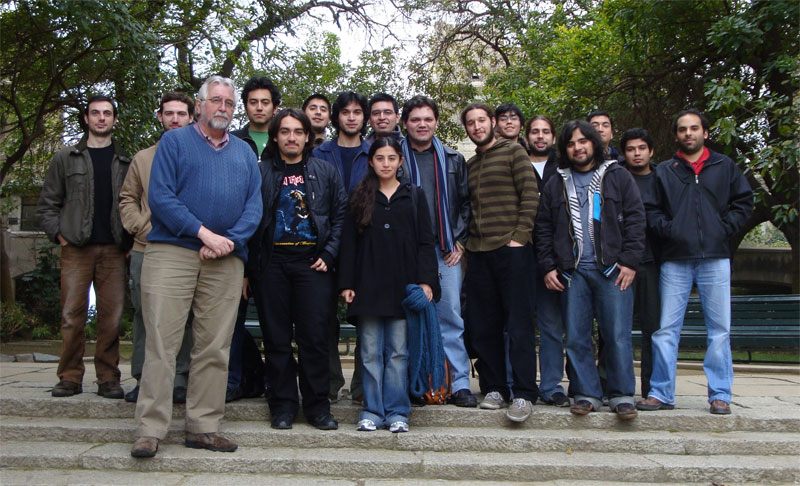
\includegraphics[width=0.8\textwidth]{images/alma-utfsm-1}\\\vspace{1cm}
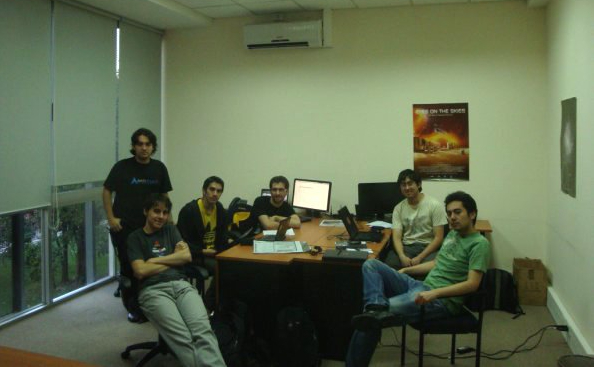
\includegraphics[width=0.8\textwidth]{images/alma-utfsm-2}\\
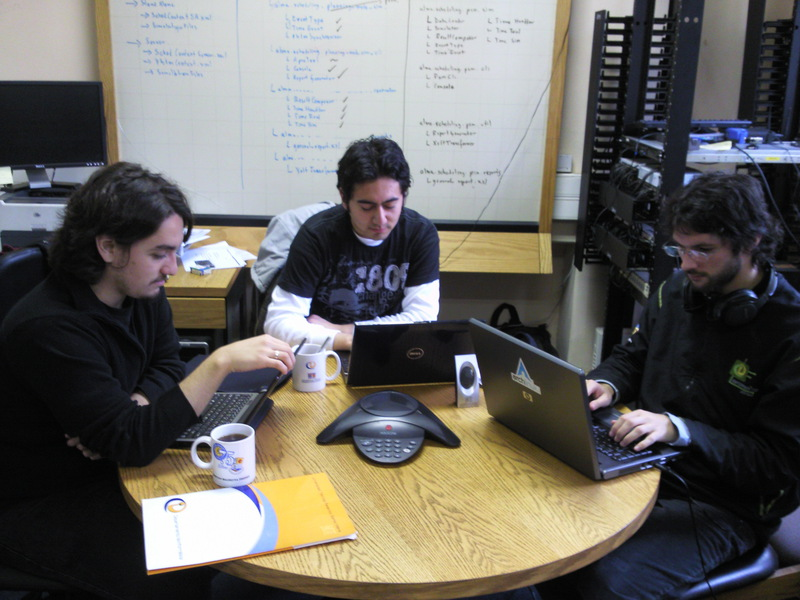
\includegraphics[width=0.8\textwidth]{images/lab_conference}\\\vspace{1cm}
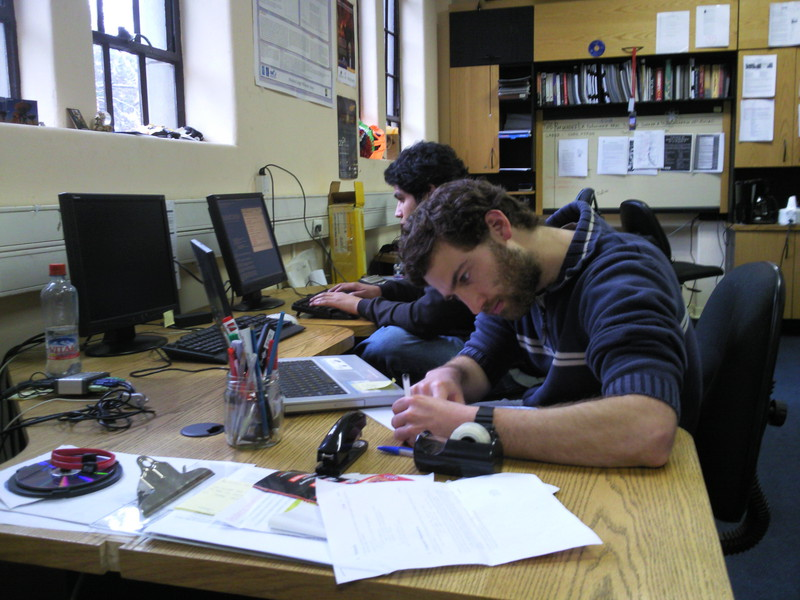
\includegraphics[width=0.8\textwidth]{images/lab_working}\\
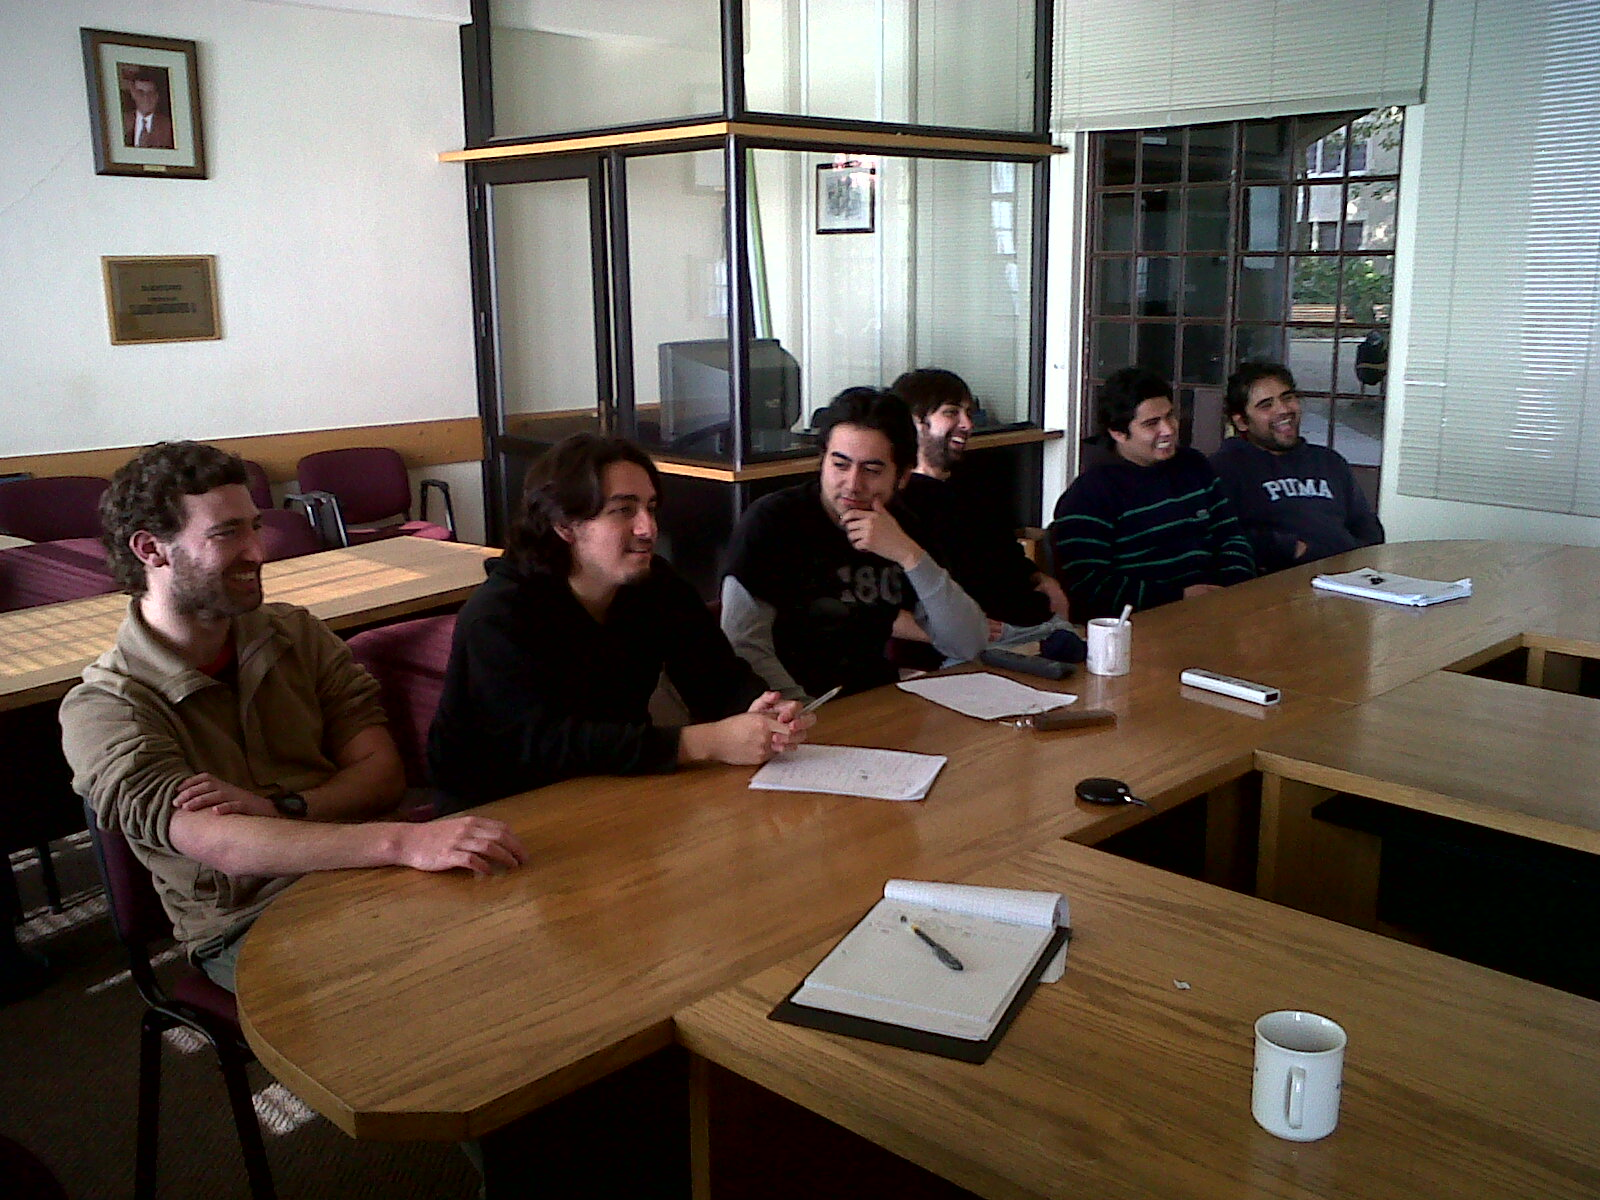
\includegraphics[width=0.8\textwidth]{images/leads1}\\\vspace{1cm}
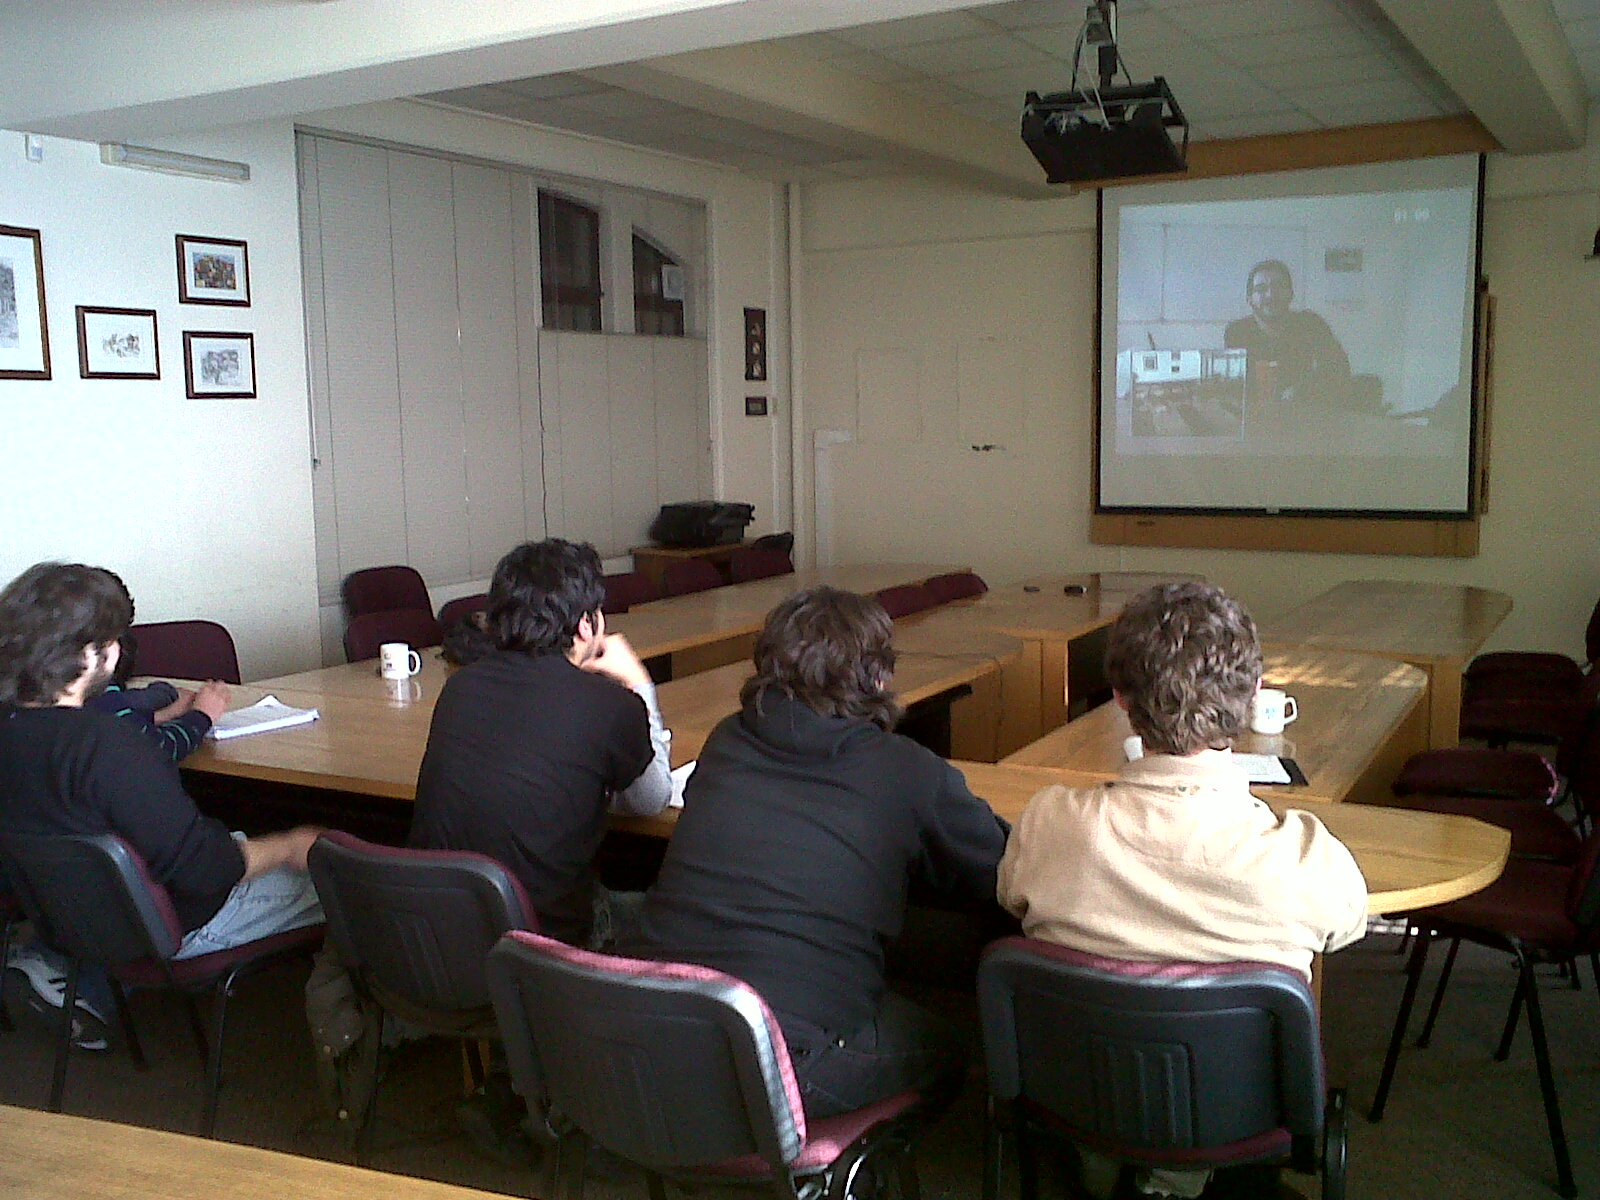
\includegraphics[width=0.8\textwidth]{images/leads2}
\end{center}
% CORRECCION &

\newpage
\subsection{Minutas de reuniones}
\subsubsubsection{ACS Weekly Meeting}
\begin{verbatim}
ACS Weekly Phone Meeting 
Date: Monday, 2010-04-12 

Attendees: 
ESO: Bogdan, Gianluca, Heiko, JosephSchwarz, 
NRAO: ArneGrimstrup, JorgeAvarias 
JSI: 
AOT: 
ALMA Chile: Ale 
UTFSM: GabrielZamora CristianMaureira 

Control contact number: +1-203-607-6471 (Passcode 203403#) 

General issues 

Alma has a promising candidate for a new board to replace the VMEs with 64 
bit architecture, to support more memory. Details from Thomas J. 
All module owners please fix their tests on 8.2 branch and HEAD. 

Ale Caproni 

Last week: 

CONTROL: Some issues with TotalPower testing, also due to STEs gotten messed up 
by other testers. 
The TP component has been changed to use the C++ API of the Bulk data libs, 
without reusing the IDL wrapper of the bulk data component. This works fine 
now, but still would like to discuss changes to the BD IDL for the long term. 
Will be at ESO early May. Things to be discussed should be added to Ale's 
Main.May2010 page.

Arne Grimstrup 

Last week: 

Continued investigation of COMP-3072 (with J. Avarias) 
problem still occurs with RHEL 5.4 version of CASA 
select is monitoring a bad file descriptor which triggers an exception 
in the TAO code. Telecon with UTFSM regarding future projects 
(with G. Chiozzi, H. Sommer, et. al.) Support 
Investigation of 64-bit test faults in NRI (H. Sommer)(with J. Avarias) 
Template method was invoking unsigned long version of getValue method 
that didn't exist Documentation for generated Python bindings (J. Kern) 
Questions regarding Python Binding Generator (J. Kern) 
Problem building ACS in INTROOT (J. Avarias) 

This week: 
Continue work on COMP-3072 
Continue work on COMP-830 

Bogdan Jeram 

Last week: 
Monday public holiday 
4 days of vacation 

Heiko Sommer 

Last week: 

Worked out HibernateDAL's usage of Archive's new archiveConfig.properties 
mechanism, together with Holger. 
Finalized 8.1 CVS logs and release notes. Pre-release of 9.0 VM. 
Discussions, e.g. TP with Ale and others 
Support, e.g. XSD validation, CDB performance fix, manager error messages, 
1 day leave 
Telecon with UTFSM about current projects 
quarterly report for ESO 

Helmut Tischer 

Last week: 
Vacation 

This week: 
COMP-2214 continuing 

Joe Schwarz 

Last week: 

Discussed problem of simultaneous use of SB by > 1 STE; change in 
lifecycle-handling needed 
Reviewed FP6 quarterly report from U. of Cambridge 
Worked on Total Power crash of Java container; suggested JNI 
debugging options for JVM runtime to Jeff and Ville, also removing
 native method invocation from class constructor (this didn't 
make any difference, however); got help from Roberto, who looked 
at logs and said he saw no bulk data issues 
Discussed CDR8 preparations w/Heiko 
Tried (and failed) to convince Brian to take Observation Control 
(not yet delivered) out of R7.1 
One day's leave 

This week: 
CDR8 preparation, ACS 9.0 planning 
Continue investigation of Total Power problem 
Return to classpath generation 

Jorge Avarias 

Last week: 

COMP-3749: ACS to introduce a new log level between DEBUG and TRACE 
Finished to make the last changes to the tests (Changed ACS_LOG_STDOUT 
from 2 to 1 new trace) 
All the tests affected by this are passing. 
Continued investigation of COMP-3072 (with A, Grimstrup) 
Fixed NRI ACS 64 bits building problems: 
The method unsigned long cdb::DAONode::getValue(char const*) 
was missing. probably some code is using unsigned long instead 
CORBA::ULong (in 32 bits they have the same length, in 64 they have not) 
Support: 
CONTROL/ACC/cppContainer crash (T. Powers) 
CONTROL/ACC/javaContainer crash, JVM is crashing with Seg. Fault 
(J. Kern, V. Suoranta) 
Problems building ACS in INTROOT (ACS is already built in ACSROOT) 
(S. Rankin) 


Matej Sekoranja 

Last week: 
HibernateDAL now skips loading all .dtd files, XMLSchema.xsd and xml.xsd so 
that Oracle's XMLTYPE checks don't get confused. 

This week: 
At CERN, but available for emergency ACS work. 

This week: 
TMCDB integration at the OSF 

UTFSM 

Last week: 

DDS Logging Service 
All the main goals are completed 
There are one pending task, write a "state of art" in this topic, for the paper 
accepted in the SPIE Meeting with people at ESO to define project objectives. 
Planning
Python support for BACI Properties 
ACS Code Generation 
ACS Windows Porting (Rodrigo and Heiko to integrate Java porting, Camillo and 
Gianluca to continue with C++ porting)
\end{verbatim}
\newpage
\subsubsubsection{OSF Coordination Meeting}

\begin{verbatim}
Date: Tue, 2010-05-18, 11:00 Chile, 9:00 Socorro, 17:00 Germany 
Attendees: 

ALMA-Chile: MatiasMora 
NRAO-Socorro: JorgeAvarias 
ESO-Garching: HeikoSommers 
UTFSM: GabrielZamora, TomasStaig, ArturoHoffstadt, CristianMaureira 
UCN: JaimePavlich 

Contact Info 
When: 11:00 Chile / 9:00 NM / 17:00 Germany 
Chile (toll free): 800532833 
International: +1 3032480281 
Access Code: 4676238 
Web Conferencing URL: http://net.globalcrossing.com/conferencing/ 

Agenda 
ALMA-CONICYT #31090034 (UTFSM) 
Projects 
ACS Windows Porting: The first version of the gcc-wrapper (gcc -> cl) is 
ready, we need to test with real examples to improve it. 
Code Generation: Luigi sent us a project proposal. Because Luigi was on
 vacations the last week, the meeting for this project is pending 
Alarms Configuration GUI: 
The project is ready, but there are some details with the redaction. 
Rules view that Tomas will fix in the week. 
Cristian Maureira and Tomas Staig will work on the documentation the 
next week. 
Official acceptance by ACS. 
Sampling System GUI: 
Juan Reyes and Cristian Maureira closed two of the three pending bugs, 
there are only one pending, that will be ready during the week. 
Official acceptance by ACS. 
ALMA-CONICYT #31080031 (AIA) 
Teams working on papers and on a new task about implementing TSP with 
their paper techniques 
HPC must to define the input framework and do some testing with TSP 
SebastianDuran and WalterFarina will be helping MatiasMora on what 
he needs for his thesis 
Second class this week Valpo. and next week Stgo. about advanced 
AI techniques 
Looking for possibilities of collaborations with MAIA-INRIA 
Summer Jobs 2010 
Pending reports! 
UCN Current Status 
Mini-ACS-Workshop from April 27th to May 10th. Funded by 
ALMA #31090026. 
Repository for UCN projects: http://goos-acs.googlecode.com 
gCCD status 
Implementing support for SBIG cameras 
Moving configuration to CDB 
gDome status 
gDome group are new students. After several intensive sessions 
they created the first version of the Dome component. 
Documentation: installation and system manuals. 
Misc 
ACS Scientific Linux distribution mirror repo here at UTFSM (ArturoHoffstadt).
\end{verbatim}

\end{document}
